% Created 2022-10-15 Sat 22:22
% Intended LaTeX compiler: pdflatex
\documentclass[12pt]{article}

%%%% settings when exporting code %%%% 

\usepackage{listings}
\lstdefinestyle{code-small}{
backgroundcolor=\color{white}, % background color for the code block
basicstyle=\ttfamily\small, % font used to display the code
commentstyle=\color[rgb]{0.5,0,0.5}, % color used to display comments in the code
keywordstyle=\color{black}, % color used to highlight certain words in the code
numberstyle=\ttfamily\tiny\color{gray}, % color used to display the line numbers
rulecolor=\color{black}, % color of the frame
stringstyle=\color[rgb]{0,.5,0},  % color used to display strings in the code
breakatwhitespace=false, % sets if automatic breaks should only happen at whitespace
breaklines=true, % sets automatic line breaking
columns=fullflexible,
frame=single, % adds a frame around the code (non,leftline,topline,bottomline,lines,single,shadowbox)
keepspaces=true, % % keeps spaces in text, useful for keeping indentation of code
literate={~}{$\sim$}{1}, % symbol properly display via latex
numbers=none, % where to put the line-numbers; possible values are (none, left, right)
numbersep=10pt, % how far the line-numbers are from the code
showspaces=false,
showstringspaces=false,
stepnumber=1, % the step between two line-numbers. If it's 1, each line will be numbered
tabsize=1,
xleftmargin=0cm,
emph={anova,apply,class,coef,colnames,colNames,colSums,dim,dcast,for,ggplot,head,if,ifelse,is.na,lapply,list.files,library,logLik,melt,plot,require,rowSums,sapply,setcolorder,setkey,str,summary,tapply},
aboveskip = \medskipamount, % define the space above displayed listings.
belowskip = \medskipamount, % define the space above displayed listings.
lineskip = 0pt} % specifies additional space between lines in listings
\lstset{style=code-small}
%%%% packages %%%%%

\usepackage[utf8]{inputenc}
\usepackage[T1]{fontenc}
\usepackage{lmodern}
\usepackage{textcomp}
\usepackage{color}
\usepackage{graphicx}
\usepackage{grffile}
\usepackage{wrapfig}
\usepackage{rotating}
\usepackage{longtable}
\usepackage{multirow}
\usepackage{multicol}
\usepackage{changes}
\usepackage{pdflscape}
\usepackage{geometry}
\usepackage[normalem]{ulem}
\usepackage{amssymb}
\usepackage{amsmath}
\usepackage{amsfonts}
\usepackage{dsfont}
\usepackage{array}
\usepackage{ifthen}
\usepackage{hyperref}
\usepackage{natbib}
\pagestyle{empty} % no page numbering
\usepackage[french]{babel}
\newcommand{\Rlogo}{\textbf{\textsf{R}}}
\newcommand{\Cpp}{C\nolinebreak\hspace{-.05em}\raisebox{.4ex}{\tiny\bf +}\nolinebreak\hspace{-.10em}\raisebox{.4ex}{\tiny\bf +}}
\usepackage{eurosym} % euro symbol
\usepackage{titlesec}
\titleformat{\section}{\large}{\thesection}{1em}{}
\titlespacing*{\section}{0pt}{0.25\baselineskip}{0.25\baselineskip}
\geometry{
left=20mm,
right=20mm,
top=20mm,
bottom=20mm
}
\hypersetup{
citecolor=[rgb]{0,0.5,0},
urlcolor=[rgb]{0,0,0.5},
linkcolor=[rgb]{0,0,0.5},
}
\RequirePackage{setspace} % to modify the space between lines - incompatible with footnote in beamer
\renewcommand{\baselinestretch}{1.1}
\usepackage{framed}
\usepackage{tocloft}
\newlength{\outerbordwidth}
\raggedbottom
\raggedright
\setlength{\outerbordwidth}{3pt}  % Width of border outside of title bars
\definecolor{shadecolor}{gray}{0.75}  % Outer background color of title bars (0 = black, 1 = white)
\definecolor{shadecolorB}{gray}{0.93}  % Inner background color of title bars
\usepackage{mdframed}
\newcommand{\resitem}[1]{\item #1 \vspace{-2pt}}
\newcommand{\resheading}[1]{
\vspace{8pt}
\parbox{\textwidth}{\setlength{\FrameSep}{\outerbordwidth}
\begin{shaded}
\setlength{\fboxsep}{0pt}\framebox[\textwidth][l]{\setlength{\fboxsep}{4pt}\fcolorbox{shadecolorB}{shadecolorB}{\textbf{\sffamily{\mbox{~}\makebox[6.762in][l]{\large #1} \vphantom{p\^{E}}}}}}
\end{shaded}
}\vspace{-5pt}
}
\newcommand{\ressubheading}[4]{
\begin{tabular*}{6.5in}{l@{\cftdotfill{\cftsecdotsep}\extracolsep{\fill}}r}
\textbf{#1} & #2 \\
\textit{#3} & \textit{#4} \\
\end{tabular*}\vspace{-6pt}}
\usepackage{bibentry}
\nobibliography*
\newcommand{\myname}[1]{\textbf{#1}}
\usepackage{url}
\usepackage{enumitem}
\date{\today}
\title{}
\hypersetup{
 colorlinks=true,
 pdfauthor={Brice Ozenne},
 pdftitle={},
 pdfkeywords={},
 pdfsubject={},
 pdfcreator={Emacs 26.3 (Org mode 9.4.6)},
 pdflang={French}
 }
\begin{document}

\begin{tabular*}{7in}{l@{\extracolsep{\fill}}r}
	\textbf{\Large Brice Ozenne} & \textbf{\today} \\
\end{tabular*}

\bigskip

\begin{minipage}{0.2\linewidth}
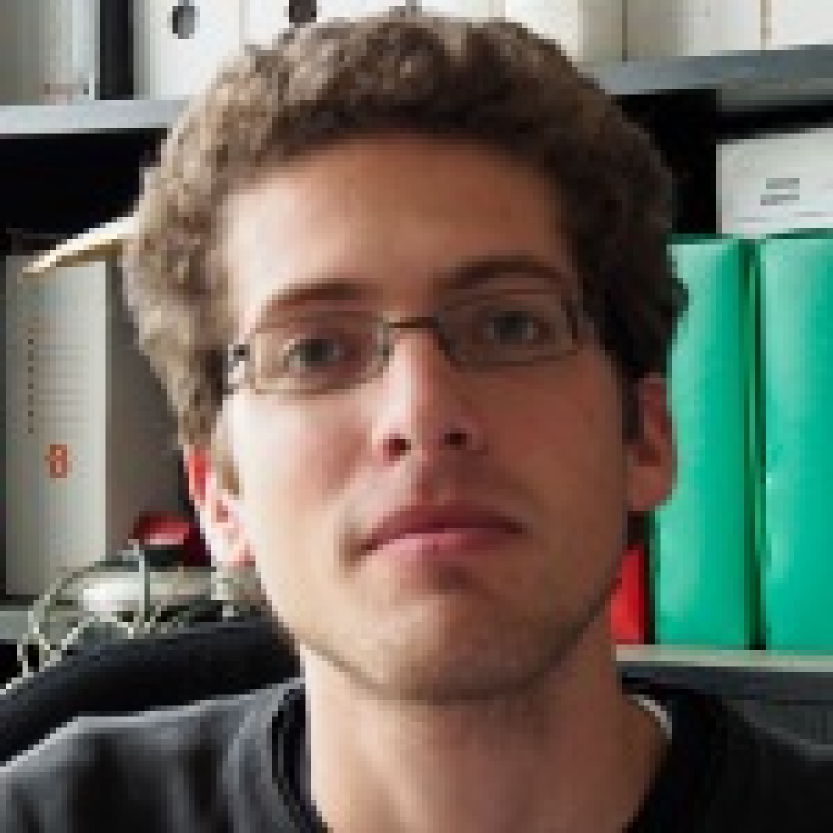
\includegraphics[width=\linewidth]{photoId.png}
\end{minipage}
\begin{minipage}{0.75\linewidth}
\begin{tabular*}{7in}{ll@{ }l}
	Nationalité&:& française  \\
	Né&:& le 8 février 1990 à Saint Hilaire du Harcouët (50)  \\
	Courriel personnel&:& \url{brice.mh.ozenne@gmail.com} \\ 
	Téléphone personnel&:& (+45) 52 328 128 \\ 
        Adresse personnelle&:& Nordre Teglkaj 18, 5 t.h., 2450 Copenhagen SV, Danemark \\
        Site internet&:& \url{https://bozenne.github.io/} \\
        Github&:& \url{https://github.com/bozenne/} \\
\end{tabular*}
\end{minipage}


\resheading{Activité de recherche}
\begin{tabular}{l@{ }l}
	Depuis octobre 2020 :& \textbf{Professeur assistant en biostatistiques} avec une position partagée entre \\ [2mm]
      & - une unité de recherche en biostatistiques \\
	& \href{https://biostat.ku.dk/staff_/?pure=en/persons/540231}{Section of Biostatistics}, University of Copenhagen \\
	& \O{}ster Farimagsgade 5, 1014 Copenhague, Danemark \\ [2mm]
	& - une unité de recherche en neuroscience \\
	& \href{https://nru.dk/index.php/staff-list/post-docs/110-brice-ozenne}{Neurobiology Research Unit} \\
	& Copenhagen University Hospital, Rigshospitalet \\
	& Building 6931, Blegdamsvej 9, DK-2100 Copenhagen, Danemark \\ [2mm]
	& où j'exerce conjointement une activité de recherche en biostatistiques, \\ 
      & de consultant en statistiques et une activité pédagogique.
\end{tabular}

\bigskip

Mon travail de recherche s'articule autour de trois thèmes:
\begin{itemize}
\item le développement de \textbf{modèles multivariés} pour l'analyse de données
en neuroscience. Principalement modèles mixed (LMM) et modèles à
variables latentes (LVM) - voir les publications
\citep{ebert2019molecular,stenbaek2017brain,fisher2017bdnf} pour des
exemples d'application. D'un point de vue méthodologique, je
m'intéresse à \textbf{l'estimation et l'inférence en petits échantillons}
\citep{ozenne2020small} ainsi qu'à développer des corrections
efficaces en présence de \textbf{tests multiples}
\citep{ozenne2022controlling}. Ces développements sont implémentés dans
les librairies R \texttt{lavaSearch2} (LVM) et \texttt{LMMstar} (LMM).
\end{itemize}

\bigskip

\begin{itemize}
\item l'analyse de données de registre en présence de \textbf{censure à droite,
risques compétitifs, et variables de confusion}, en particulier pour
comparer l'efficacité de traitements préventifs de maladies
cardiovasculaires (publications
\cite{staerk2018standard,staerk2017resumption,staerk2016ischaemic}). En
utilisant des résultats de la \textbf{théorie semi-paramétrique}, j'ai
développé un estimateur robuste basé sur plusieurs modèles de
régressions et utilisé sa fonction d'influence pour obtenir sa
distribution asymptotique \citep{ozenne2020estimation}. Cette méthode
est implémentée dans la fonction \texttt{ate} de la librairie R
\texttt{riskRegression}. Voir aussi \citep{scheike2022efficient} pour un
travail plus théorique sur l'efficacité d'estimateurs issus du
modèle de Fine and Gray.
\end{itemize}

\bigskip

\begin{itemize}
\item l'extension des \textbf{méthodes de comparaison par paires} (GPC) aux
données censurées \citep{peron2016extension}. Les GPC permettent
d'analyser simultanément plusieurs critères de jugements et donc
d'évaluer la balance bénéfice-risque d'un traitement. Une
application typique est de proposer une statistique reflétant à la
fois les gains en survie et les effets secondaires de traitements
anti-cancéreux (publications \citep{peron2016net} et
\citep{peron2016assessment}). Je m'intéresse par exemple à la théorie
des U-statistiques pour obtenir la distribution asymptotique de
certains estimateurs implémentés dans la librairie R \texttt{BuyseTest}
(\citep{ozenne2021asymptotic}).
\end{itemize}

\bigskip

\section*{\emph{Autres domaines d'intérêt en statistiques:}}
\label{sec:org174576b}
\begin{itemize}
\item Spline de lissages et modélisation fonctionnelle
\item Inférence causale et régimes de traitement dynamiques
\item Essais cliniques séquentiels
\item Inférence statistique après sélection
\end{itemize}
\resheading{Compétences}
\section*{\emph{Linguistiques}}
\label{sec:orgd173631}
Français (langue maternelle), anglais (courant), danois (intermédiaire), notions d'italien.

\section*{\emph{Logicielles}}
\label{sec:orge1f410b}
Bonne connaissance de \Rlogo{}, \LaTeX{} et \href{https://orgmode.org/}{orgmode}. \\
Utilisation courante mais basique de \Cpp{}, lisp (pour \href{https://www.gnu.org/software/emacs/}{GNU Emacs}),
git/github et inkscape.
\resheading{Formation universitaire et parcours de recherche}
\begin{tabular}{l@{ }l}
2015 - 2020 :& \textbf{Post-doctorat en biostatistiques} avec une position partagée entre: \\
\multicolumn{2}{l}{- \emph{l'Université de Copenhague}: rechercheur et enseignant à l'école doctorale de médicine.}  \\
\multicolumn{2}{l}{- \emph{le CHU de Copenhague (NRU)}: consultant et responsable de l'analyse de données}\\
\multicolumn{2}{l}{ \hphantom{le CHU de Copenhague (NRU): } au sein du projet \href{https://np.nru.dk/}{Neuropharm}.}\\
\end{tabular}
Développement de modèle à variables latents en neuroimagerie (librarie R \texttt{lavaSearch2}) ainsi que d'estimateurs robustes pour l'analyse de données de registre (librarie R \texttt{riskRegression}).

\bigskip

\begin{tabular}{l@{ }l}
2012 - 2015 : & \textbf{Doctorat en biostatistiques}, Université Lyon 1. \\
\multicolumn{2}{l}{\emph{Directeur/Co-directeur}: Pr. Delphine Maucort-Boulch / Pr. Norbert Nighoghossian} \\ 
\multicolumn{2}{l}{Sujet: \href{https://tel.archives-ouvertes.fr/tel-01233049/document}{modélisation statistique pour le pronostic de patients atteints d’un Accident Vasculaire Cérébral}} \\ 
\multicolumn{2}{l}{\hphantom{Sujet:} Développement d'outils de segmentation d'image et de prédiction appliqués à l'AVC.}\\
\multicolumn{2}{l}{\hphantom{Sujet:} Le produit final étant une prédiction personnalisée de l'extension du volume de l'AVC}\\
\multicolumn{2}{l}{\hphantom{Sujet:} à l'admission du patient à l'hopital.} \\ [3mm]
\end{tabular}

\begin{tabular}{l@{ }l}
2012 : & \textbf{Stage de master 2}, Hospices Civils de Lyon. \\
\multicolumn{2}{l}{\emph{Encadrant}: Pr. Delphine Maucort-Boulch} \\ 
\multicolumn{2}{l}{Sujet: mise en place d’un critère IRM de reperfusion lors d'un AVC} \\ 
\multicolumn{2}{l}{\hphantom{Sujet:} Le stage a permis de proposer un critère de reperfusion basé sur trois mesures IRM} \\
\multicolumn{2}{l}{\hphantom{Sujet:} du niveau de perfusion et de le valider au regard de critères cliniques.} \\  [3mm]
\end{tabular}

\begin{tabular}{l@{ }l}
2009 - 2012 : & \textbf{Formation d'ingénieur avec spécialisation en statistiques} à École Centrale de Lyon \\ 
              & \textbf{Erasmus} à l'Université Politecnico di Milano (2nd semestre 2011) \\
              & \textbf{Master en biostatistiques} à l'Université Lyon 1 en double diplôme (\href{http://mastersantepublique.univ-lyon1.fr/webapp/website/website.html?id=3124911&pageId=215838}{M2 B3S}). \\
\end{tabular}

\resheading{Enseignement et encadrement d'étudiants}
Enseignement (CM : cours magistral, TD : travaux dirigés):

\medskip

Doctorants en santé:

\begin{tabular}{r@{ }l}
2021 - 2022 : & \href{http://publicifsv.sund.ku.dk/~jufo/RepeatedMeasures2019.html}{Analyse statistique de données répétées}. CM et TD (6h et 18h). \\
            : & Outils statistiques pour l'épidémiologie. Responsable CM, TD (10h et 18h). \\
            : & Introduction aux statistiques. CM, TD (3h et 3h). \\
2015 - 2020 : & \href{http://publicifsv.sund.ku.dk/~jufo/RepeatedMeasures2019.html}{Analyse statistique de données répétées}. TD (18h). \\
\end{tabular}

\bigskip

Etudiants de master de statistiques:

\begin{tabular}{l@{ }l}
2016 - 2017 : & Modèles d'équations structurelles. CM (2h). \\
\end{tabular}

\bigskip

Etudiants de master en santé publique:

\begin{tabular}{l@{ }l}
2014 - 2015 : & \href{https://clarolineconnect.univ-lyon1.fr/resource/open/file/2733301}{Modèles de Survie}. TD (18h).\\
2013 - 2015 : & \href{https://clarolineconnect.univ-lyon1.fr/resource/open/file/2733304}{Statistique bayésienne}. TD (6h).\\
\end{tabular}


\bigskip

Exposés pédagogiques pour chercheurs en neuroscience sur des
outils/problématiques statistiques:
\begin{itemize}
\item \href{https://bozenne.github.io/doc/Talks/2017-XNRU-power.pdf}{Do we need more power?} (\href{https://www.nru.dk/images/News/NeurobiologyResearchUnit-Christmas-symposium2017.pdf}{NRU Christmas Symposium 2017}).
\item \href{https://bozenne.github.io/doc/Talks/2018-XNRU-DAGs.pdf}{To adjust or not adjust, that is the question} (NRU Christmas Symposium 2018).
\item \href{https://bozenne.github.io/doc/Talks/2019-XNRU-multcomp.pdf}{A refresher on multiple comparisons}? (\href{https://nru.dk/index.php/news-menu/279-nru-christimas-symposium-2019}{NRU Christmas Symposium 2019}).
\end{itemize}

\bigskip

Co-encadrant d'étudiant en \textbf{master 2}: 

\medskip

\begin{tabular}{l@{ }l@{ }l}
2014 &:& Ceren Tozlu \\
\multicolumn{3}{l}{Comparaison de méthodes de classification pour la prédiction du devenir des tissus lors} \\ 
\multicolumn{3}{l}{d'un AVC \citep{tozlu2019comparison}.} \\ [3mm]
2019 &:& Alice Brouquet-Laglaire \\
\multicolumn{3}{l}{Comparaison de méthodes d’inférence dans le cadre des comparaisons par paires généralisées.} \\ [3mm]
\end{tabular}

\resheading{Financement}
\begin{tabular}{l@{ }l}
2017-2019: MARIE CURIE Individual Fellowships (200 000\euro) \\
2017-2020: Lundbeck Fellowships (140 000\euro) \\

\end{tabular}

\clearpage

\resheading{Production scientifique}
\section*{\emph{Publications (méthodologiques)}}
\label{sec:org6561b82}

\begin{enumerate}
   \item \bibentry{scheike2022efficient}
   \item \bibentry{ozenne2022controlling}
   \item \bibentry{ozenne2021asymptotic}
   \item \bibentry{peron2021correcting}
   \item \bibentry{cantagallo2021new}
   \item \bibentry{ozenne2020small}
   \item \bibentry{verbeeck2020evaluation}
   \item \bibentry{ozenne2020estimation}
   \item \bibentry{norgaard2019preprocessing}
   \item \bibentry{ozenne2017riskregression}
   \item \bibentry{peron2016extension}
   \item \bibentry{ozenne2015precision}
   \item \bibentry{ozenne2015spatially}
 \end{enumerate}

\section*{\emph{Développement logiciel (librairies pour le logiciel \href{https://www.r-project.org/}{R})}}
\label{sec:orgd909762}
\begin{minipage}{0.01\textwidth}
\hspace{\fill}
\end{minipage}
\begin{minipage}{0.92\textwidth}
\begin{itemize}
\item \textbf{BuyseTest} (Créateur et mainteneur) : Comparisons par paires
généralisées. Implémentation de la méthode décrite dans
\citep{peron2016extension,peron2021correcting}. Disponible sur le \href{https://cran.r-project.org/web/packages/BuyseTest/index.html}{CRAN}
et sur \href{https://github.com/bozenne/BuyseTest}{Github}.

\item \textbf{lavaSearch2} (Créateur et mainteneur) : Inférence et outils
diagnostiques dans les modèles à variables latentes
(\cite{ozenne2020small,ozenne2022controling}). Disponible sur
le \href{https://cran.r-project.org/web/packages/lavaSearch2/index.html}{CRAN} et sur \href{https://github.com/bozenne/lavaSearch2}{Github}. .

\item \textbf{LMMstar} (Créateur et mainteneur) : Modèles mixtes linéaires:
formulation marginale avec differentes structures de
variance-covariance residuelle et outils d'inférence statistique
associés'. Disponible sur le \href{https://cran.r-project.org/web/packages/LMMstar/index.html}{CRAN} et sur \href{https://github.com/bozenne/LMMstar}{Github}. .

\item \textbf{riskRegression} (Contributeur) : Calculateur du risque
d'évènenement en présence de risques compétitifs. Implémentation de
la méthode décrite dans \cite{ozenne2017riskregression} et
\cite{ozenne2020estimation}. Disponible sur le \href{https://cran.r-project.org/web/packages/riskRegression/index.html}{CRAN} et sur \href{https://github.com/tagteam/riskRegression}{Github}.
\end{itemize}
\end{minipage}

\bigskip

Librairie pour le logiciel \href{https://www.gnu.org/software/emacs/}{emacs}:
\begin{itemize}
\item \textbf{emacs-config} (Créateur et mainteneur) : configuration facilitant
l'intéraction avec R/C++/orgmode/latex/git. Disponible sur sur
\href{https://github.com/bozenne/emacs-config}{Github}.
\end{itemize}

\pagebreak[3]

\section*{\emph{Publications (applications cliniques)}}
\label{sec:org6010ede}

\begin{enumerate}[resume]
   \item \bibentry{nasser2022reliability}
   \item \bibentry{armand2022brain}
   \item \bibentry{kohler2022concurrent}
   \item \bibentry{armand2022acute}
   \item \bibentry{armand2022brain}
   \item \bibentry{fisher2022emotional}
   \item \bibentry{beaman2022blood}
   \item \bibentry{drummond2022psilocybin}
   \item \bibentry{larsen2022impact}
   \item \bibentry{mcculloch2022lasting}
   \item \bibentry{ip2021eeg}
   \item \bibentry{madsen2021psilocybin}
   \item \bibentry{joergensen2021default}
   \item \bibentry{brandt2021reward}
   \item \bibentry{dea2021brain}
   \item \bibentry{ip2021pretreatement}
   \item \bibentry{hoghe2021MAMA}
   \item \bibentry{raval2021single}
   \item \bibentry{hogsted2021stress}
   \item \bibentry{donovan2021effects}
   \item \bibentry{lee2020absolute}
   \item \bibentry{hansen2020visual}
   \item \bibentry{spies2020common}
   \item \bibentry{larsen2020oral}
   \item \bibentry{thystrup2020severity}
   \item \bibentry{dam2020hot}x
   \item \bibentry{hjordt2020psychometric}
   \item \bibentry{beliveau2020structure}
   \item \bibentry{madsen2020single}
   \item \bibentry{ozenne2019individualized}
   \item \bibentry{ebert2019molecular}
   \item \bibentry{madsen2019psychedelic}
   \item \bibentry{tozlu2019comparison}
   \item \bibentry{ip2018pre}
   \item \bibentry{borgsted2018amygdala}
   \item \bibentry{hjordt2018self}
   \item \bibentry{foged2018verbal}
   \item \bibentry{staerk2018standard}
   \item \bibentry{hjordt2017season}
   \item \bibentry{beliveau2017high}
   \item \bibentry{stenbaek2017brain}
   \item \bibentry{staerk2017resumption}
   \item \bibentry{fisher2017bdnf}
   \item \bibentry{foged2017safety}
   \item \bibentry{peron2016net}
   \item \bibentry{staerk2016ischaemic}
   \item \bibentry{peron2016assessment}
   \item \bibentry{ozenne2015evaluation}
   \item \bibentry{hermitte2013very}
 \end{enumerate}

\pagebreak[3]
\resheading{Relecture d'article}
J'ai relu des articles pour Biometrics, Statistics in Medicine,
International Journal of Biostatistics, and BMC medical reasearch
methodology. Voir mon \href{https://publons.com/researcher/1214277/brice-maxime-hugues-ozenne/}{profile publons} pour plus d'informations.


\clearpage

\resheading{Conférences}
Présentations orales lors de conférences internationales: 
\smallskip

\begin{tabular}{l@{ }l@{ }l}
2014 &:& Image segmentation using a spatially regularized mixture model \\
&& \href{https://www.biometricsociety.org/meetings-events/ibcs/}{IBC}, Florence, Italie \\
2015 &:& \href{https://r2015-grenoble.sciencesconf.org/66037}{MRIaggr : un package pour la gestion et le traitement de données multivariées d'imagerie} \\
&& Rencontres R, Grenoble, France \\
2016 &:& \href{http://cmstatistics.org/RegistrationsV2/COMPSTAT2016/viewSubmission.php?in=440&token=29584n1s18p97n65o7p1r5n36sopq0n4}{Penalized latent variable models} \\
&& Computational statistics, Oviedo, Espagne \\
2017 &:& Assessing treatment effects on registry data in presence of competing risks \\ 
&& \href{http://www.iscb2017.info/}{ISCB}, Vigo, Espagne \\
2019 &:& Generalized pairwise comparisons for right-censored time to event outcomes \\
&& \href{https://publicifsv.sund.ku.dk/~safjr2019/}{Survival analysis for junior researcher}, Copenhague, Danemark \\
2020 &:& Robust estimation of the average treatment effects in presence of right-censoring \\
&& and competing risks \\
&& \href{http://www.cmstatistics.org/conferences.php}{CMStatistics}, Londres, Angleterre \\
\end{tabular}

\bigskip

Responsable de session ("chairman"):

\smallskip

\begin{tabular}{l@{ }l@{ }l}
2019 &:& Mathematical Statistics \\
&& \href{https://publicifsv.sund.ku.dk/~safjr2019/}{Survival analysis for junior researcher}, Copenhague, Danemark
\end{tabular}

\bigskip

Organisation d'une formation ("Workshop"):
\begin{tabular}{l@{ }l@{ }l}
2021 &:& Analysis of repeated measurements with mixed models using the R package LMMstar (1h+3h) \\
&& Methods Week, Karolinska institute, Stockholm, Sweden
\end{tabular}

\smallskip


\bibliographystyle{plainnat}

\nobibliography{publicationBO}
\end{document}